

\chapter{Softwarearchitektur der bestehenden Software}

    Analysemethoden der Informatik für Software sind in der Regel für die verschiedenen Design-Phasen einer Software entwickelt worden. Eine von mir durchgeführte Recherche ergab,
    dass sich Analyse-Tools und Methoden für bestehende Software vor Allem darauf fokussieren die Performance, Speichermanagement und Benutzererfahrung zu bewerten.
    Die Architektur einer Software spielt dabei eine untergeordnete Rolle.
    Für die Neuentwicklung der bestehenden Software werden im Folgenden die Klassen und Objekte sowie ihre Wechselwirkungen dargestellt und anschließend analysiert und bewertet.
    \\
    In einem C\# - Projekt sind UI und Logik in getrennten Dateien implementiert. XAML- Dateien sind eine angepasste Form von XML-Dateien. Sie legen fest wie etwas gerendert wird während
    XAML.CS- Dateien die dahinterliegende Buisiness-Logik abbilden.
    Am Beispiel des Haupt-GUI des Programms soll der prinzipielle Aufbau gezeigt werden. Wegen der Komplexizität wird der Umfang jedoch nicht für das gesamte Programm fortgesetzt.
    \subsection {Lagerverwaltung 3.0}
    \begin{itemize}
        \item Die Datei \verb|App.xaml.cs| ist der Einstiegspunkt des Programms.
        \item Die Datei \verb|App.xaml| erzeugt ein Objekt der Apllication Klasse und erzeugt ein Dictionary mit den Ressourcen der Anwendung. Als Startup-URL ist die Datei \verb |MainWindow.xaml| festgelegt.
        \item In \verb|MainWindow.xaml| wird:
        \begin{itemize}
            \item Das Hauptfenster gerendert.
            \item Objekte und Variablen initialisiert, die dem Lager zugeordnet sind:
            \begin{itemize}
                \item Ein Objekt \verb|inventory| der Klasse \verb|Inventory| für das Inventar mit \verb|null| initialisiert.
                \item Ein Objekt \verb|storageMatrix| von der Klasse \verb|PalletMatrix| erzeugt.
                \item Ein Object \verb|commissionMatrix| von der Klasse \verb|PalletMatrix| erzeugt.
                \item Ein Objekt \verb|mobileRobot| von der Klasse \verb |MobileRobot| erzeugt.
                \item Außerdem eine Variable \verb|lastCupRead| vom Datentyp \verb|ushort| (16-Bit-Ganzzahl, vorzeichenlos) mit 0 initialisiert.
            \end{itemize}
            \item Objekte und Variablen initialisiert, die dem ABB Controller zugeordnet sind:
            \begin{itemize}
                \item Ein Objekt \verb|commands| von der Klasse \verb|controllerCommandList|.
                \item Ein Objekt \verb|controllerProperties| von der Klasse \verb|RobotControllerProperties|.
                \item Ein Objekt \verb|controllerBase| von der Klasse \verb|RobotControllerBas|, mit dem Initialisierungswert \verb|null|.
                \item Ein Objekt \verb|controllerSim| von der Klasse \verb|RobotSimulator|.
            \end{itemize}
        \end{itemize}
        Im Constructor der Klasse werden der ModBus und der Roboter Controller initialisiert, die Produktlistegeladen und gerendert.
        Daten des Lagers und des turtlebots sowie Comissionsdaten werden geladen und anschließend das Inventar gerendert.
    \end{itemize}
        Abb. 1 zeigt einen Screenshot des Hauptbildschirm des Programms. Es ist in 7 wesentliche Teile eingeteilt:
    \begin{figure}[h]
        \label{fig:figure}
        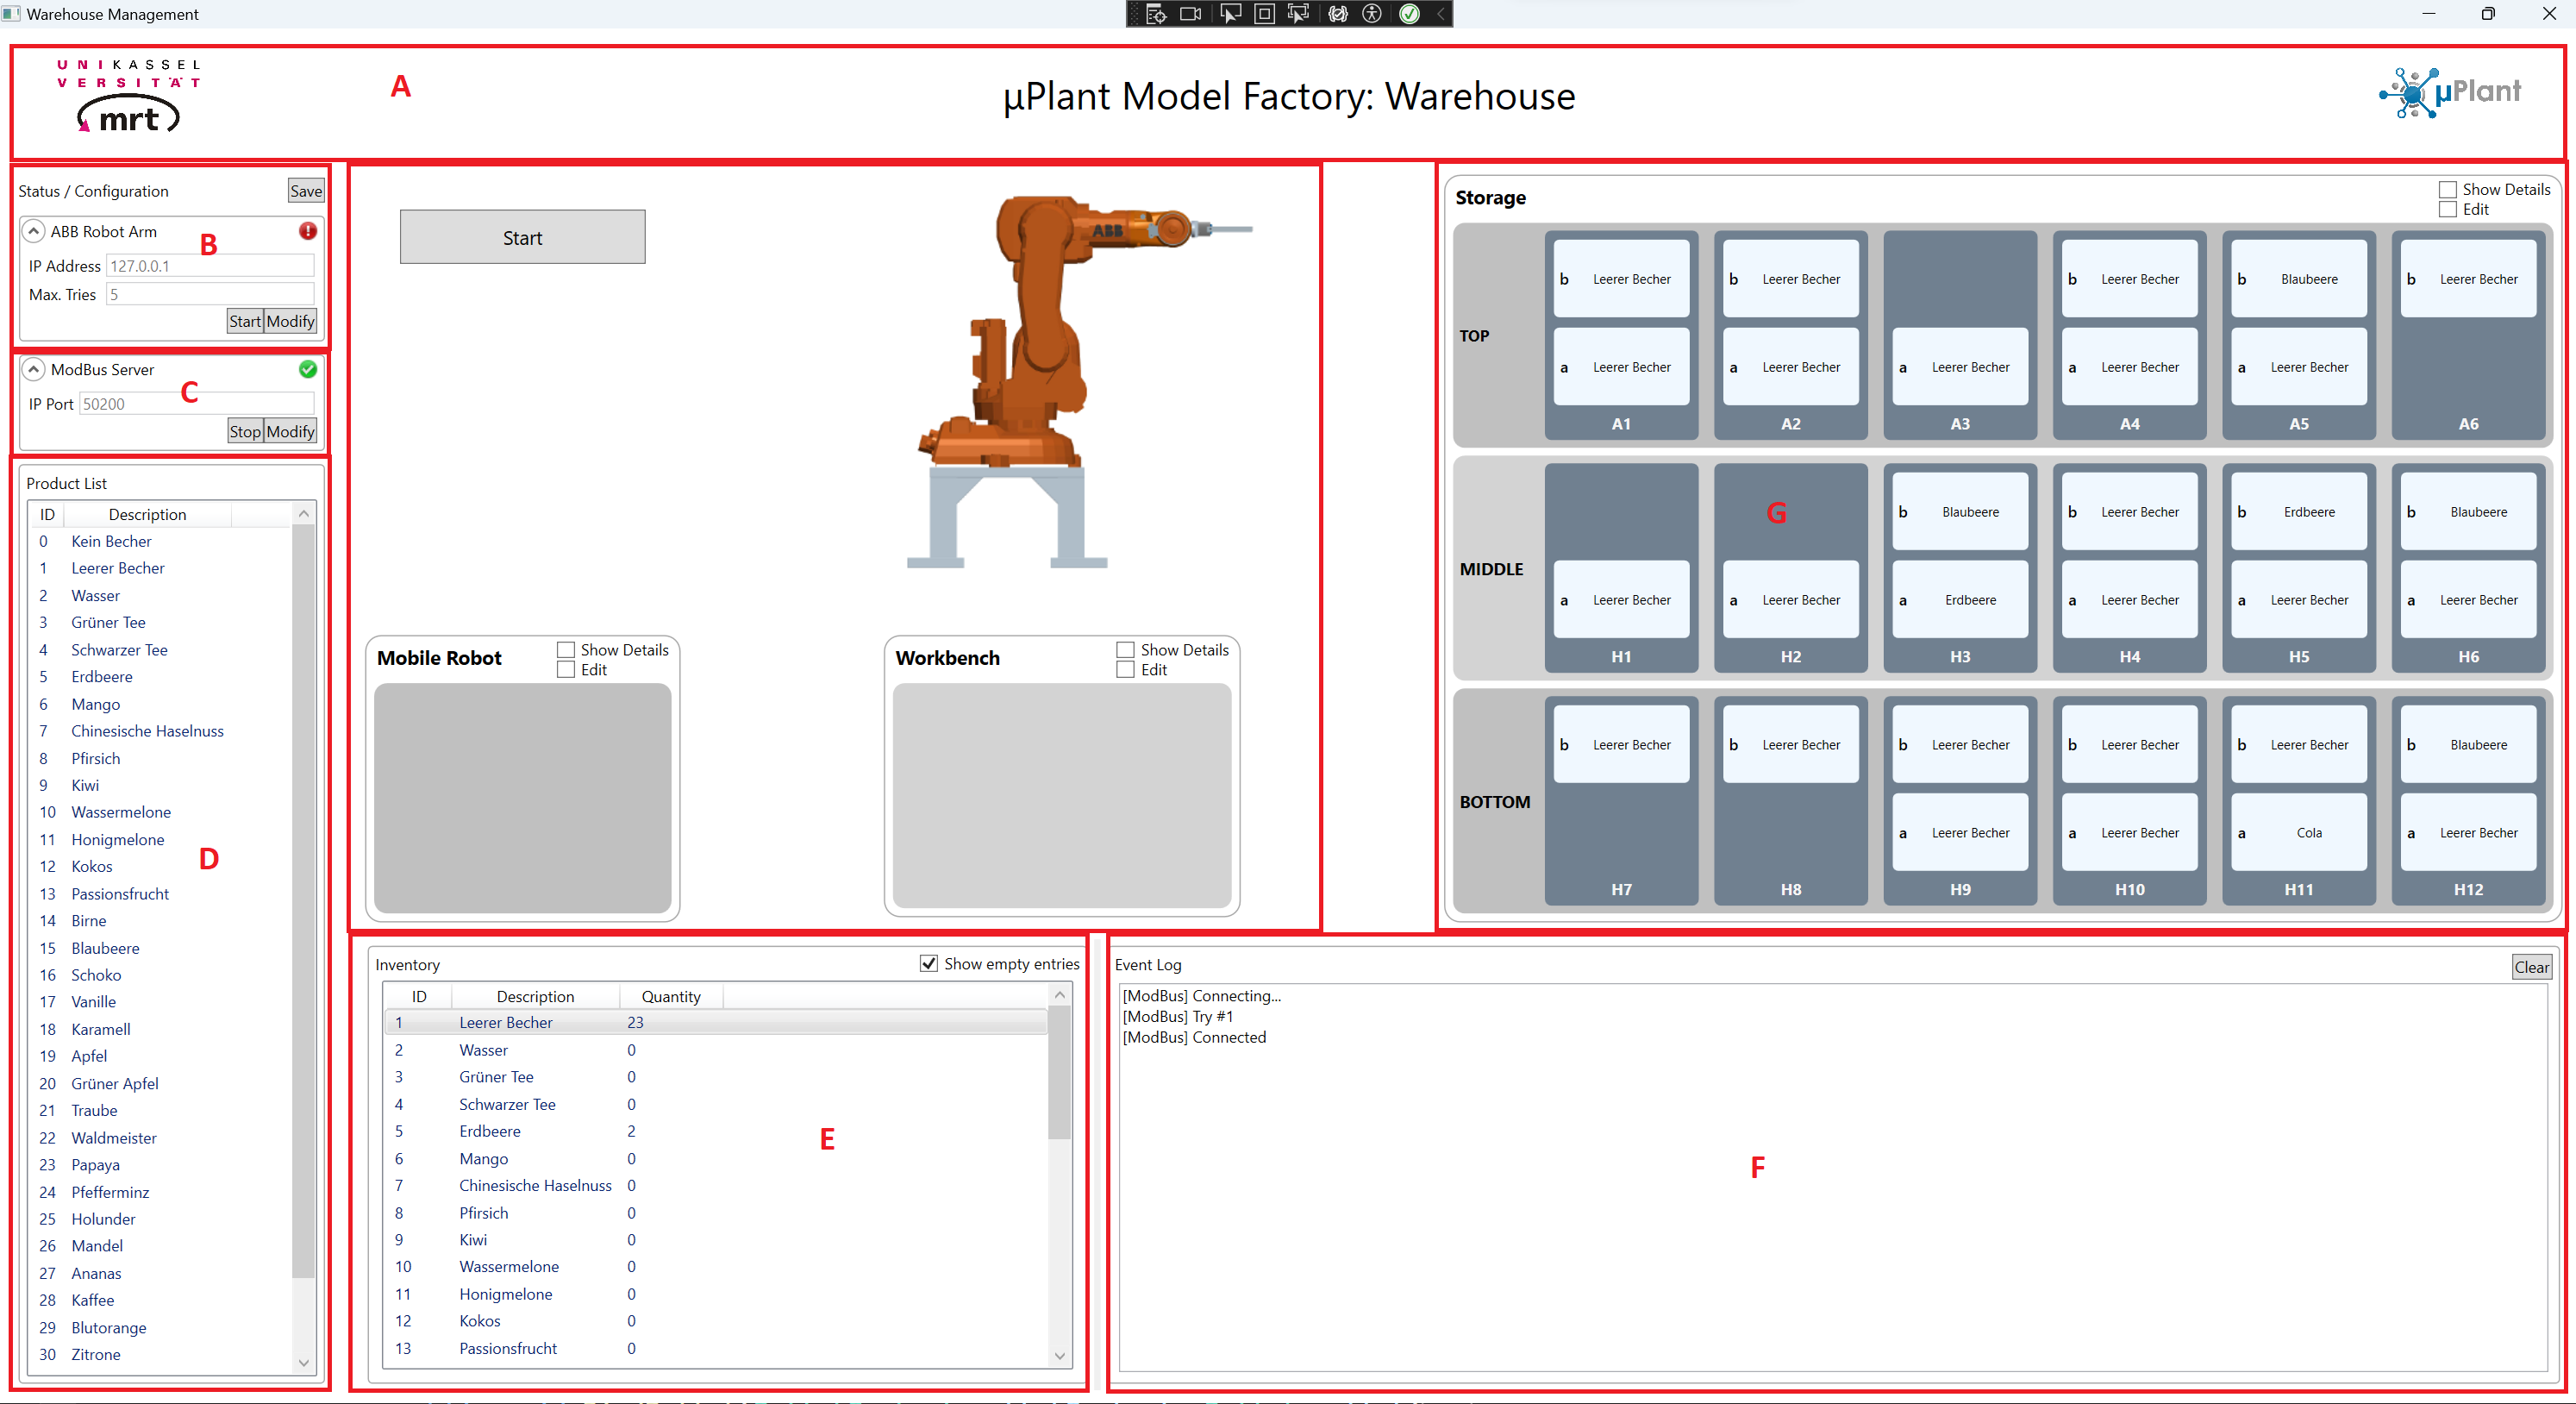
\includegraphics[width = \textwidth ]{Bilder/LV_Startbildschirm}
        \caption[Ansicht des Startbildschirms]%
        {\small Startbildschirm der Anwendung, zur besseren Beschreibung sind die Bedienbereiche rot umrandet und mit
        Buchstanben gekennzeichnet}
        \centering
    \end{figure}

    \begin{figure}[h]
        \label{fig:figure2}
        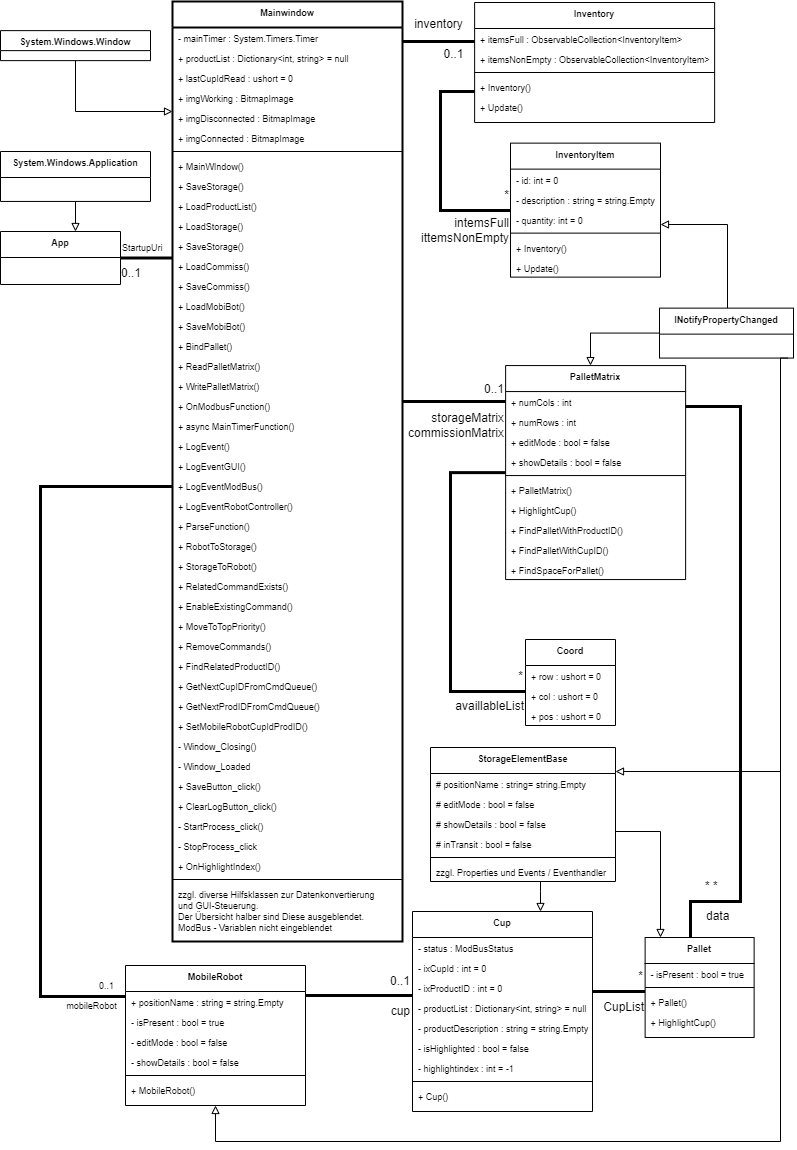
\includegraphics[width = \textwidth ]{Bilder/LV_Klassendiagramm_Datenmodell}
        \caption[Klassendiagramm Datenmodells ]%
        {\small Klassendiagramm der MainWindow-Klasse mit vererbenden- und Datenmodell - Klassen }
        \centering
    \end{figure}

    \begin{figure}[h]
        \label{fig:figure3}
        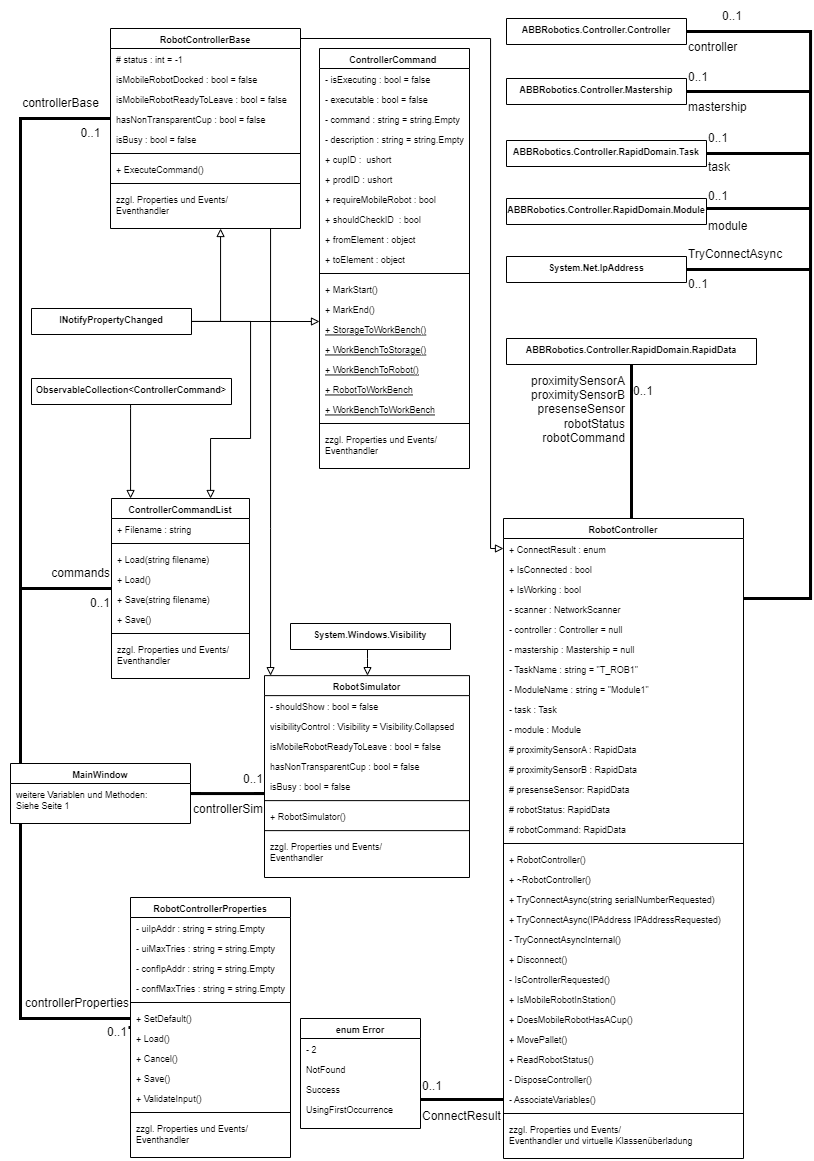
\includegraphics[width = \textwidth ]{Bilder/LV_Klassendiagramm_ABBController}
        \caption[Klassendiagramm ABB Controller ]%
        {\small Klassendiagramm der MainWindow-Klasse mit Klassen aus dem ABB Controllerframework. }
        \centering
    \end{figure}

    \begin{figure}[h]
        \label{fig:figure4}
        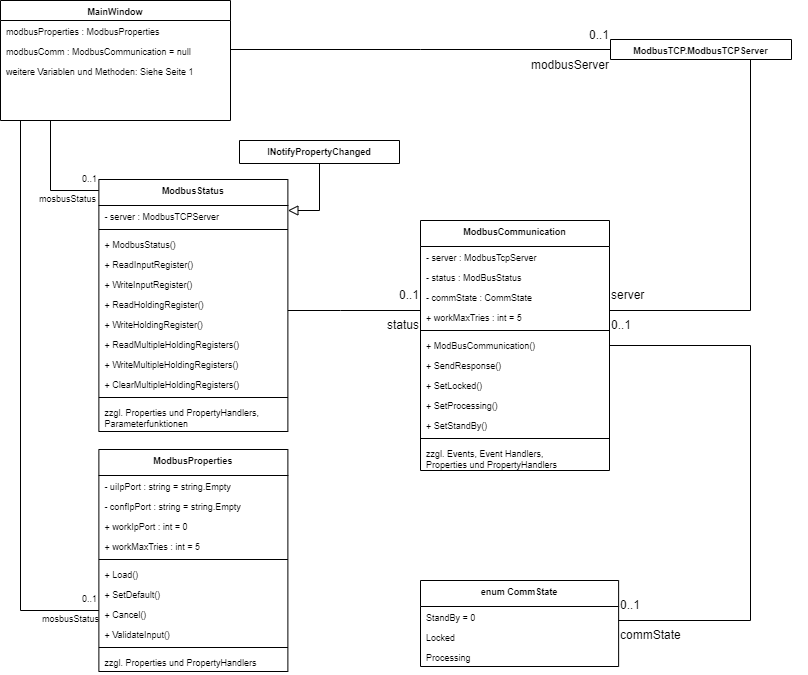
\includegraphics[width = \textwidth ]{Bilder/LV_Klassendiagramm_Modbus}
        \caption[Klassendiagramm Modbus ]%
        {\small Klassendiagramm der MainWindow-Klasse mit Mosbus-Klassen }
        \centering
    \end{figure}

    \begin{figure}[h]
        \label{fig:figure5}
        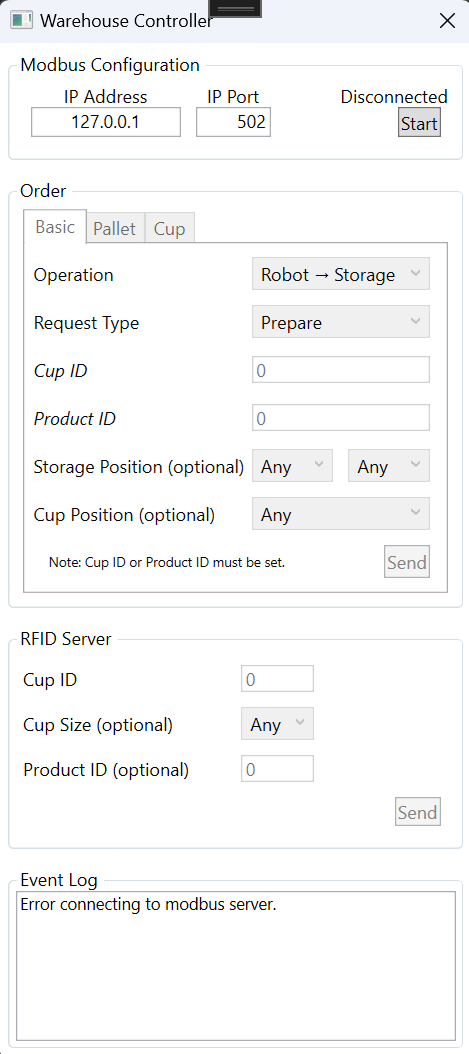
\includegraphics[width = \textwidth ]{Bilder/Controller_Startbildschirm}
        \caption[Ansicht des Controller- Startbildschirm ]%
        {\small Ansicht des Controller Startbildschirms. }
        \centering
    \end{figure}

    \begin{figure}[h]
        \label{fig:figure6}
        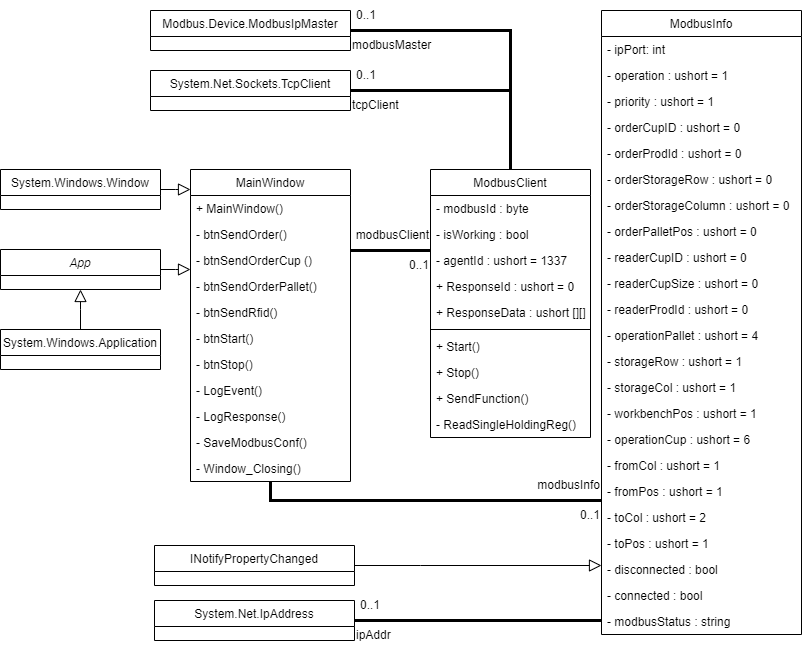
\includegraphics[width = \textwidth ]{Bilder/C_Klassendiagramm}
        \caption[Klassendiagramm des Controllers ]%
        {\small Klassendiagramm des Warehouse-Controllers mit allen vererbenden Klassen jedoch ohne Klassen die
        lediglich Datentypen konvertieren.}
        \centering
    \end{figure}

    \begin{figure}[h]
        \label{fig:figure7}
        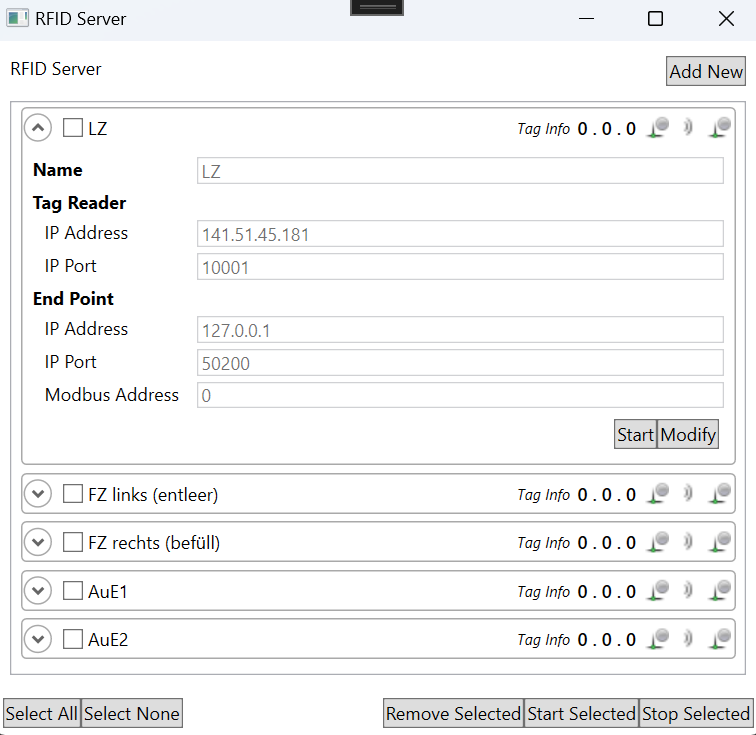
\includegraphics[width = \textwidth ]{Bilder/RFIDServer_Bildschirm}
        \caption[Startbildschirm des Programms "RFID-Server" ]%
        {\small Startbildschirm des Programms "RFID-Server"}
        \centering
    \end{figure}

\begin{figure}[h]
        \label{fig:figure8}
        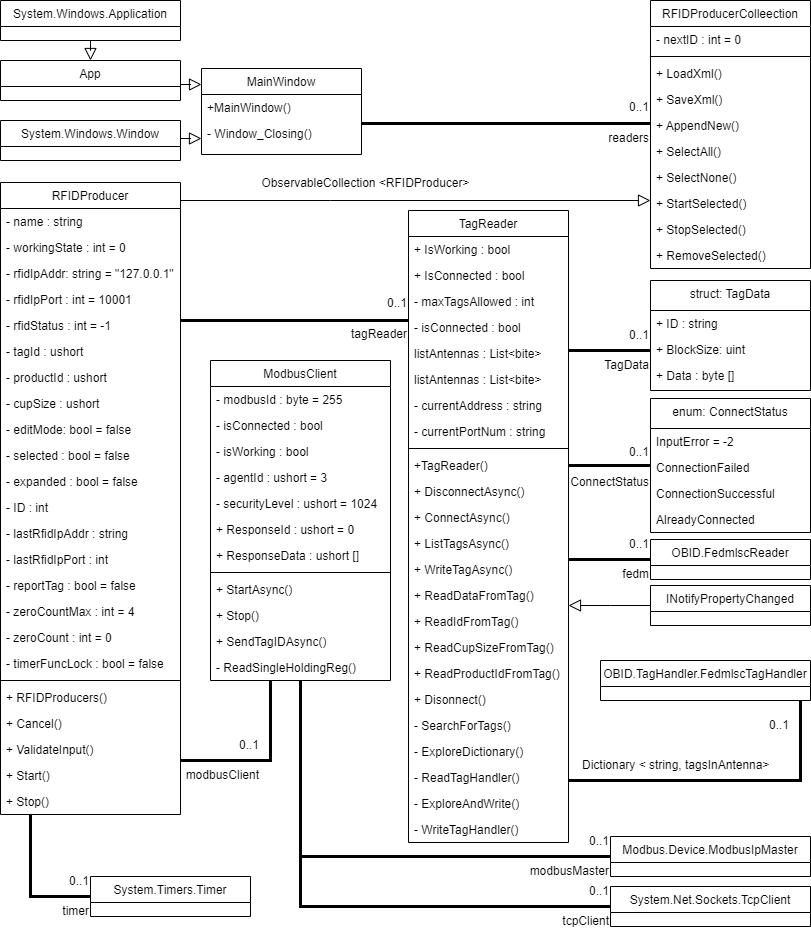
\includegraphics[width = \textwidth ]{Bilder/RFID_Klassendiagramm}
        \caption[Klassendiagramm des Programms "RFID-Server" ]%
        {\small Klassendiagramm des Programms "RFID-Server" mit allen vererbenden Klassen jedoch ohne solche die
        lediglich Typen konvertieren.}
        \centering
    \end{figure}


    \begin{itemize}
        \item Der rote , mit "1" markierte Bereich im Startbildschirm dient dazu die Verbindungsdaten zum ModBus zu konfigurieren. Über entsprechende Taste kann die Eingabe der beiden Felder aktiviert/deaktiviert werden. Über die Start-Taste wird die VErbindung hergestellt.
        An der Stelle des sichtbaren roten Ausrufezeichen-Symbol wird ein grüner Haken sichtbar, wenn die Verbindung korrekt hergestellt wurde.
        \item Der blaue, mit "2" markierte Bereich dient dazu gesondert den ModBus-Port einzustellen.
        \item Der grüne, mit "3" markierte Bereich ist eine Listenansicht, in der jedes mögliche Produkt mit seiner zugeordneten ID abgebildet ist.
        Die Liste ermöglicht dem Benutzer einen schnellen Überblick über mögliche Produkte.
        \item Der gelbe, mit "4" markierte Bereich ist die Übersicht über das aktuelle Geschehen. Im linken, unteren Bereich ist der Lagerplatz des mobilen Roboters symbolisiert.
        Im rechten, unteren Bereich ist der Lagerplatz der Werkbank symbolisiert. Beide Symboliken verfügen über je einen Lagerplatz, wobei die real doppelte Ausführung der Werkbank nicht umgesetzt wurde.
        \item die violetten Bereiche "5" und "6" bilden die Visualisierung des Lagers. In Bereich 6 sind die 18 Lagerslots so dargestellt wie das reale Regal aufgebaut ist. Einzig die Lagerort-Bezeichnung ist anders.
        Im Bereich "5" werden alle möglichen Produkte in einer Liste mit der gelagerten Menge angezeigt. Wahlweise können alle Produkte ausgeblendet werden, die keine Bestand haben.
        Mit Klick auf ein Produkt, egal ob im Bereich "5" oder "6", werden alle passenden Einträge farblich hervorgehoben, sodass auf einen Blick erkennbar ist, wo die Lagermenge im Lager wirklich abgebildet ist.
        \item Im grünen, mit "7" gekennzeichneten Bereich ist ein Eventlogger implementiert. Wann immer ein für den Benutzer relevantes Ereignis eintritt, wird hier eine entsprechende Meldung angezeigt.
    \end{itemize}
    \subsubsection{Lagerelemente}
    Die bestehende Software dient dazu Lagerpakete vom mobilen Roboter auf die Werkbank oder ins Lager zu bewegen. Oder alle möglichen Kombinationen davon.
    Das Konzept der $\mu$Plant beschränkt sich dabei auf eine Palette, die so ausgeführt ist, dass der Greifer des Industrieroboters sie sicher bewegen kann. Im Wesentlichen ist es ein Quader mit zwei seitlichen Längsnuten.
    Eine Palette enthält zwei senkrechte Bohrungen, die es ermöglichen je einen Becher aufzunehmen.\\
    Ein Becher ist ein transparentes, zylindrisches Gefäß aus Acrylglas mit einem Absatz, der etwa mittig in der Höhe angebracht ist. Dadurch können die Becher einzeln vom Greifer bewegt werden.

    \subsection {RFID Server}

    \subsection {Controller}

